\documentclass[aspectratio=169]{beamer}

% ==== Theme & basic look ====
\usetheme{Madrid}
\usecolortheme{seahorse}
\setbeamertemplate{navigation symbols}{}
\setbeamertemplate{footline}[frame number]

% Packages for mathematics  
\usepackage{amsmath}  
\usepackage{amsfonts}  
\usepackage{amssymb}  
\usepackage{CJKutf8}
% Support for \Tilde macro used throughout
\providecommand{\Tilde}[1]{\tilde{#1}}
\providecommand{\proofname}{Proof}
% Custom environments removed for debugging

% Math shorthand and vector symbols
\newcommand{\grad}{\nabla}
\newcommand{\EE}{\mathbb{E}}
\newcommand{\dd}{\mathrm{d}}
\newcommand{\kbT}{k_B T}
\newcommand{\vx}{\mathbf{x}}
\newcommand{\R}{\mathbb{R}}

% Bold vector/time-indexed variables
\newcommand{\vxz}{\mathbf{x}_0}
\newcommand{\vxt}{\mathbf{x}_t}
\newcommand{\alpt}{\alpha_t}
\newcommand{\sigt}{\sigma_t}
\newcommand{\veps}{\boldsymbol{\epsilon}}
\newcommand{\vF}{\mathbf{F}}

% Title page details:   
\title[Understanding normalizing flows]{Understanding normalizing flows from a mathematical view}  
\author{Pipi Hu}  
\institute[BIMSA]{Beijing Institute of Mathematical Sciences and Applications}  
\date{\today}  

\pgfdeclareimage[width=2cm]{logo}{../figures/logo.png}
\logo{\pgfuseimage{logo}}

% Outline slide (moved to later; avoid frame before \begin{document})

\setbeamertemplate{navigation symbols}{}
\AtBeginSection[]  
{  
    \begin{frame}<beamer>{Outline}         
        \tableofcontents[currentsection]  
    \end{frame}  
}  
  
\AtBeginSubsection[]  
{  
    \begin{frame}<beamer>{Outline}         
        \tableofcontents[currentsection,currentsubsection]  
    \end{frame}  
}  

\begin{document}  
  
% Title slide  
\begin{frame}  
  \titlepage  
\end{frame}  

\begin{frame}{Feynman's words}
\centering
    What I cannot create, I do not understand.
\end{frame}
  
% Presentation slides  

\section{Introduction: Normalizing Flows in the Generative Modeling Landscape}

\begin{frame}{Three perspectives so far}
\textbf{Recap of previous lectures:}
\begin{itemize}
    \item \textbf{Diffusion models} (Lecture 1): start from data, add Gaussian noise via an SDE, and learn the \emph{score} $\nabla_{\vx}\log p_t(\vx)$ (or equivalent $\epsilon$/$x_0$ models) to run a reverse-time denoising process.
    \item \textbf{Flow matching} (Lecture 2): prescribe a path of marginals $(p_t)_{t\in[0,1]}$ and learn a velocity field $v_\theta(x,t)$ whose ODE transports a simple prior into the data distribution.
    \item \textbf{VAEs} (Lecture 3): introduce latent variables $z$, optimize an ELBO, and use an encoder $q_\phi(z\mid x)$ and decoder $p_\theta(x\mid z)$ trained with the reparameterization trick.
\end{itemize}
\vspace{0.5em}
\textbf{Question:} Can we build generative models that are \emph{both} probabilistically principled (like VAEs/diffusions) and allow \emph{exact} likelihoods and fast sampling?
\end{frame}

\begin{frame}{Core idea of normalizing flows}
\textbf{Normalizing flows:} learn an invertible mapping $T_\theta:\R^d\to\R^d$ that pushes a simple base distribution (e.g.\ $\mathcal{N}(0,I)$) to the data distribution.
\begin{itemize}
    \item \textbf{Forward (generation):} sample $z\sim p_Z$ and set $x = T_\theta(z)$.
    \item \textbf{Inverse (density evaluation):} given $x$, compute $z = T_\theta^{-1}(x)$ and
    \[
      \log p_\theta(x) = \log p_Z(z) + \log\left|\det \frac{\partial T_\theta^{-1}(x)}{\partial x}\right|.
    \]
    \item \textbf{Training:} maximize exact log-likelihood $\mathbb{E}_{p_{\text{data}}}[\log p_\theta(x)]$, just as in classical maximum-likelihood modeling.
\end{itemize}
\textcolor{red}{Key challenge:} design $T_\theta$ so that both $T_\theta^{-1}$ and the Jacobian determinant are tractable in high dimensions.
\end{frame}

\begin{frame}{Flows vs. VAEs, diffusion, and flow matching}
\textbf{Comparison with VAE:}
\begin{itemize}
    \item VAE optimizes an \emph{approximate} ELBO and uses a stochastic encoder $q_\phi(z\mid x)$.
    \item Flows avoid variational approximation: the mapping is deterministic and invertible, and $\log p_\theta(x)$ is computed exactly.
\end{itemize}

\textbf{Comparison with diffusion / flow matching:}
\begin{itemize}
    \item Diffusion and flow matching describe a \emph{continuous-time path} $(p_t)$ and learn a score or velocity field, then integrate an SDE/ODE at inference time.
    \item Normalizing flows instead parameterize the \emph{end-to-end transport map} as a finite composition of invertible layers; sampling is a single forward pass with no stochastic integration.
\end{itemize}

\textbf{This lecture:} develop the change-of-variables formula, study discrete flows (autoregressive and coupling-based), continuous flows (Neural ODE / FFJORD), and conditional normalizing flows.
\end{frame}

\section{Preliminary: Change of Variables and Jacobian}

\begin{frame}{Normalizing: Change of Variables Theorem}
Given a bijective transformation $T: \mathbb{R}^d \to \mathbb{R}^d$ with inverse $T^{-1}$, and probability densities $p_X(x)$ and $p_Y(y)$, we have:
\begin{equation}
    p_Y(y) = p_X(T^{-1}(y)) \left|\det \frac{\partial T^{-1}(y)}{\partial y}\right|
\end{equation}
where $\frac{\partial T^{-1}(y)}{\partial y}$ is the Jacobian matrix of the inverse transformation.

\begin{itemize}
    \item \textcolor{red}{Key insight}: We can transform simple distributions into complex ones
    \item \textcolor{red}{Challenge}: Computing determinants is computationally expensive
    \item \textcolor{red}{Solution}: Design transformations with tractable Jacobians
\end{itemize}
\end{frame}

\begin{frame}{Proof of the Change of Variables Formula (Part 1)}
\textbf{Theorem}: For bijective $T: \mathbb{R}^d \to \mathbb{R}^d$ with inverse $T^{-1}$,
\begin{equation}
    p_Y(y) = p_X(T^{-1}(y)) \left|\det \frac{\partial T^{-1}(y)}{\partial y}\right|
\end{equation}

\begin{block}{Proof}
Let $A \subset \mathbb{R}^d$ be any measurable set. Then:
\begin{equation}
    \int_A p_Y(y) dy = \mathbb{P}(Y \in A) = \mathbb{P}(X \in T^{-1}(A))
\end{equation}

The key insight is that we can relate the probability measures through the transformation $T$.
\end{block}
\end{frame}

\begin{frame}{Proof of the Change of Variables Formula (Part 2)}
\small
\begin{block}{Proof (Cont)}
Using the change of variables formula for integrals:
\begin{equation}
    \mathbb{P}(X \in T^{-1}(A)) = \int_{T^{-1}(A)} p_X(x) dx = \int_A p_X(T^{-1}(y)) \left|\det \frac{\partial T^{-1}(y)}{\partial y}\right| dy
\end{equation}

Since this holds for any measurable set $A$, we have:
\begin{equation}
    p_Y(y) = p_X(T^{-1}(y)) \left|\det \frac{\partial T^{-1}(y)}{\partial y}\right|
\end{equation}

\textbf{Key insight}: The Jacobian determinant accounts for how the transformation changes volumes in the space.
\end{block}

\begin{alertblock}{Remark}
    This change of variables formula is fundamental to all normalizing flows and ensures that probability mass is conserved during transformations.
\end{alertblock}
\end{frame}

\begin{frame}{Flows: Neural blocks for invertible transformations}
A normalizing flow is a sequence of invertible transformations:
\begin{equation}
    \mathbf{x}_0 \xrightarrow{T_1} \mathbf{x}_1 \xrightarrow{T_2} \mathbf{x}_2 \xrightarrow{T_3} \cdots \xrightarrow{T_K} \mathbf{x}_K
\end{equation}

The probability density transforms as:
\begin{equation}
    \log p(\mathbf{x}_K) = \log p(\mathbf{x}_0) + \sum_{k=1}^K \log \left|\det \frac{\partial T_k}{\partial \mathbf{x}_{k-1}}\right|
\end{equation}

\textbf{Goal}: Learn $T_1, T_2, \ldots, T_K$ such that $p(\mathbf{x}_K)$ matches the data distribution.
\end{frame}

\section{Autoregressive Flows}

\begin{frame}{Autoregressive Transformations}
An autoregressive transformation processes variables in order:
\begin{equation}
    y_i = \tau(x_i; \mathbf{h}_i)
\end{equation}
where $\mathbf{h}_i = h_i(x_1, x_2, \ldots, x_{i-1})$ is a function of previous variables.

\textbf{Key properties}:
\begin{itemize}
    \item \textcolor{green}{Triangular Jacobian}: $\frac{\partial y_i}{\partial x_j} = 0$ for $j > i$
    \item \textcolor{green}{Efficient determinant}: $\det J = \prod_{i=1}^d \frac{\partial y_i}{\partial x_i}$
    \item \textcolor{green}{Easy inverse}: Can be computed sequentially
\end{itemize}
\end{frame}

\begin{frame}{Masked Autoregressive Flow (MAF)}
MAF uses neural networks with masking to ensure autoregressive structure:
\begin{equation}
    y_i = x_i \odot \exp(\alpha_i) + \beta_i
\end{equation}
where $\alpha_i, \beta_i$ are outputs of a masked neural network.

\textbf{Masking strategy}:
\begin{itemize}
    \item Input mask: Only allow connections from $x_1, \ldots, x_{i-1}$ to $\alpha_i, \beta_i$
    \item Ensures $\frac{\partial y_i}{\partial x_j} = 0$ for $j \geq i$
    \item Jacobian is lower triangular by construction
\end{itemize}
\end{frame}


\begin{frame}{Inverse Autoregressive Flow (IAF)}
IAF is the inverse of MAF:
\begin{equation}
    x_i = (y_i - \beta_i) \odot \exp(-\alpha_i)
\end{equation}

\textbf{Key differences from MAF}:
\begin{itemize}
    \item \textcolor{blue}{Fast sampling}: Can generate samples in parallel
    \item \textcolor{red}{Slow density evaluation}: Requires sequential computation
    \item \textcolor{blue}{Fast training}: When used for variational inference
\end{itemize}

\textbf{Training strategy}: Use IAF for fast sampling, MAF for fast density evaluation.
\end{frame}

\begin{frame}{TarFlow: Transformer-based Autoregressive Flow}
TarFlow is a Transformer-based variant of Masked Autoregressive Flows (MAFs) designed for high-resolution image synthesis.

\textbf{Key Features}:
\begin{itemize}
    \item \textcolor{blue}{Autoregressive Transformer Blocks}: Stack of autoregressive Transformer blocks on image patches
    \item \textcolor{blue}{Alternating Autoregression}: Alternates autoregression direction between layers
    \item \textcolor{blue}{End-to-End Training}: Direct modeling and generation of pixels
    \item \textcolor{blue}{State-of-the-art Performance}: First standalone normalizing flow to match diffusion model quality
\end{itemize}

\textbf{Applications}: High-resolution image synthesis, conditional generation, density estimation.
\end{frame}

\begin{frame}{TarFlow: Architecture and Processing}
\textbf{Overall Architecture}:
\begin{itemize}
    \item \textcolor{green}{Input Processing}: Images divided into patches, each patch embedded into $D$-dimensional vectors
    \item \textcolor{green}{Transformer Layers}: $T$ autoregressive transformer layers with causal attention
    \item \textcolor{green}{Permutation Strategy}: Alternating permutations between layers for bidirectional modeling
    \item \textcolor{green}{Output}: Final latent representation $z^T$ in standard Gaussian space
\end{itemize}

\textbf{Layer-wise Processing}:
\begin{equation}
    x \xrightarrow{f^0} z^1 \xrightarrow{f^1} z^2 \xrightarrow{f^2} \cdots \xrightarrow{f^{T-1}} z^T
\end{equation}

\textbf{Each Layer $t$ Consists of}:
\begin{enumerate}
    \item \textcolor{blue}{Permutation}: $\tilde{z}^t = \pi^t(z^t)$
    \item \textcolor{blue}{Autoregressive Transformation}: $z^{t+1} = f^t(\tilde{z}^t)$
\end{enumerate}

\textbf{Key Design Principles}:
\begin{itemize}
    \item \textcolor{red}{Causal Attention}: Each patch can only attend to previous patches
    \item \textcolor{red}{Permutation Alternation}: Even/odd layers use different permutation orders
    \item \textcolor{red}{Bidirectional Modeling}: Captures dependencies in both directions over multiple layers
\end{itemize}
\end{frame}


\begin{frame}{TarFlow: Autoregressive Transformation with Permutations}
\textbf{Forward Transformation (Data to Latent)}:
\begin{align}
    \tilde{z}^t &= \pi^t(z^t) \\
    z_i^{t+1} &= \begin{cases}
        \tilde{z}_i^t & i = 0 \\
        (\tilde{z}_i^t - \mu_i^t(\tilde{z}_{<i}^t)) \odot \exp(-\alpha_i^t(\tilde{z}_{<i}^t)) & i > 0
    \end{cases}
\end{align}

\textbf{Inverse Transformation (Latent to Data)}:
\begin{align}
    \tilde{z}_i^t &= \begin{cases}
        z_i^{t+1} & i = 0 \\
        z_i^{t+1} \odot \exp(\alpha_i^t(\tilde{z}_{<i}^t)) + \mu_i^t(\tilde{z}_{<i}^t) & i > 0
    \end{cases} \\
    z^t &= (\pi^t)^{-1}(\tilde{z}^t)
\end{align}

\textbf{Key Properties}:
\begin{itemize}
    \item \textcolor{blue}{Causal Dependencies}: $\mu_i^t$ and $\alpha_i^t$ depend only on $\tilde{z}_{<i}^t$
    \item \textcolor{blue}{Permutation}: $\pi^t$ alternates between layers for bidirectional modeling
    \item \textcolor{blue}{Autoregressive}: Maintains autoregressive structure for exact likelihood
\end{itemize}
\end{frame}

\begin{frame}{TarFlow: Training Objective and Loss}
\textbf{Complete Training Loss}:
\begin{equation}
    \min_f 0.5\|z^T\|_2^2 + \sum_{t=0}^{T-1} \sum_{i=1}^{N-1} \sum_{j=0}^{D-1} \alpha_i^t(z^t_{<i})_j
\end{equation}

\textbf{Loss Components}:
\begin{itemize}
    \item \textcolor{green}{Square Term}: $0.5\|z^T\|_2^2$ - L2 norm of final latent representation
    \item \textcolor{green}{Linear Terms}: $\sum_{t=0}^{T-1} \sum_{i=1}^{N-1} \sum_{j=0}^{D-1} \alpha_i^t(z^t_{<i})_j$ - Sum of all scale parameters
\end{itemize}

\textbf{Training Process}:
\begin{itemize}
    \item \textcolor{blue}{Forward Pass}: Transform data $x$ through $T$ layers to get $z^T$
    \item \textcolor{blue}{Loss Computation}: Compute both square term and sum of $\alpha$ parameters
    \item \textcolor{blue}{Backpropagation}: Update parameters to minimize the combined loss
\end{itemize}

\textbf{Key Insight}: The loss simply consists of a square term and a sum of linear terms.
\end{frame}

\begin{frame}{TarFlow: Base Sampling Process}
\textbf{Standard Sampling Procedure}:
\begin{enumerate}
    \item \textcolor{blue}{Latent Sampling}: Sample $\mathbf{z} \sim p_0$ from prior distribution (e.g., standard Gaussian)
    \item \textcolor{blue}{Inverse Flow}: Apply inverse transformation $f^{-1}$ to get initial sample $\mathbf{y}$
\end{enumerate}

\textbf{Mathematical Formulation}:
\begin{equation}
    \mathbf{z} \sim p_0, \quad \mathbf{y} := f^{-1}(\mathbf{z})
\end{equation}

\textbf{Complete Sampling Process}:
\begin{align}
    \mathbf{z} &\sim \mathcal{N}(0, I) \\
    \mathbf{y} &= f_1^{-1} \circ f_2^{-1} \circ \ldots \circ f_T^{-1}(\mathbf{z})
\end{align}

\textbf{Key Properties}:
\begin{itemize}
    \item \textcolor{green}{Exact Sampling}: No approximation errors in the sampling process
    \item \textcolor{green}{Deterministic Inverse}: Each layer has exact inverse transformation
    \item \textcolor{green}{Sequential Processing}: Must process layers in reverse order
\end{itemize}
\end{frame}

\begin{frame}{TarFlow: Conditional Generation with Guidance}
\textbf{Guidance Mechanism}: Similar to classifier-free guidance in diffusion models.

\textbf{Guided Reverse Function}:
\begin{equation}
    \hat{\mathbf{z}}^t = \mathbf{z}^{t+1} \odot \exp(\hat{\boldsymbol{\alpha}}^t(\hat{\mathbf{z}}_{<t}^t; c, w)) + \hat{\boldsymbol{\mu}}^t(\hat{\mathbf{z}}_{<t}^t; c, w)
\end{equation}

\textbf{Guided Parameters}:
\begin{align}
    \hat{\boldsymbol{\mu}}^t(\hat{\mathbf{z}}_{<t}^t; c, w) &= (1 + w)\boldsymbol{\mu}^t(\hat{\mathbf{z}}_{<t}^t; c) - w\boldsymbol{\mu}^t(\hat{\mathbf{z}}_{<t}^t; \emptyset) \\
    \hat{\boldsymbol{\alpha}}^t(\hat{\mathbf{z}}_{<t}^t; c, w) &= (1 + w)\boldsymbol{\alpha}^t(\hat{\mathbf{z}}_{<t}^t; c) - w\boldsymbol{\alpha}^t(\hat{\mathbf{z}}_{<t}^t; \emptyset)
\end{align}

\textbf{Notation}:
\begin{itemize}
    \item \textcolor{green}{$c$}: Class condition (e.g., "cat", "dog")
    \item \textcolor{green}{$\emptyset$}: Unconditional prediction (obtained by dropping class labels)
    \item \textcolor{green}{$w$}: Guidance weight (controls strength of conditioning)
\end{itemize}


\begin{alertblock}{Remark}
    The guidance mechanism in TarFlow is directly inspired by classifier-free guidance in diffusion models, providing similar flexibility for conditional generation.
\end{alertblock}
\end{frame}

\begin{frame}{TarFlow: Training for Conditional Generation}
\textbf{Training Strategy}:
\begin{itemize}
    \item \textcolor{blue}{Class-conditional Training}: Train with class labels $c$ to get $\boldsymbol{\mu}^t(\cdot; c)$ and $\boldsymbol{\alpha}^t(\cdot; c)$
    \item \textcolor{blue}{Unconditional Training}: Randomly drop class labels during training to get $\boldsymbol{\mu}^t(\cdot; \emptyset)$ and $\boldsymbol{\alpha}^t(\cdot; \emptyset)$
    \item \textcolor{blue}{Joint Training}: Both conditional and unconditional predictions learned simultaneously
\end{itemize}

\textbf{Guidance Weight Effects}:
\begin{itemize}
    \item \textcolor{green}{$w = 0$}: Standard conditional generation
    \item \textcolor{green}{$w > 0$}: Stronger conditioning, better mode-seeking
    \item \textcolor{green}{$w < 0$}: Weaker conditioning, more diversity
\end{itemize}

\textbf{Applications}:
\begin{itemize}
    \item \textcolor{red}{Class-conditional Generation}: Generate images of specific classes
    \item \textcolor{red}{Style Transfer}: Control artistic style during generation
    \item \textcolor{red}{Attribute Control}: Control specific attributes (color, shape, etc.)
\end{itemize}

\textbf{Advantages over Traditional Methods}:
\begin{itemize}
    \item \textcolor{blue}{Flexible Control}: Trade-off between diversity and mode-seeking
    \item \textcolor{blue}{No Additional Models}: Uses only the trained TarFlow model
    \item \textcolor{blue}{Consistent Quality}: Maintains high sample quality with guidance
\end{itemize}
\end{frame}


\section{Coupling Layers}

\begin{frame}{Affine Coupling Layers}
Split the input $\mathbf{x}$ into two parts: $\mathbf{x}_A$ and $\mathbf{x}_B$.

\textbf{Forward transformation}:
\begin{align}
    \mathbf{y}_A &= \mathbf{x}_A \\
    \mathbf{y}_B &= \mathbf{x}_B \odot \exp(\alpha(\mathbf{x}_A)) + \beta(\mathbf{x}_A)
\end{align}

\textbf{Jacobian}:
\begin{equation}
    J = \begin{pmatrix}
        I & 0 \\
        \frac{\partial \mathbf{y}_B}{\partial \mathbf{x}_A} & \text{diag}(\exp(\alpha(\mathbf{x}_A)))
    \end{pmatrix}
\end{equation}

\textbf{Determinant}: $\det J = \prod_{i \in B} \exp(\alpha_i(\mathbf{x}_A))$
\end{frame}

\begin{frame}{Real NVP: Real-valued Non-volume Preserving}
Real NVP uses alternating coupling layers:
\begin{enumerate}
    \item \textbf{Checkerboard masking}: Alternate which dimensions are transformed
    \item \textbf{Channel-wise masking}: For images, alternate RGB channels
\end{enumerate}

\textbf{Architecture}:
\begin{itemize}
    \item ResNet blocks for $\alpha$ and $\beta$ networks
    \item Batch normalization between layers
    \item Multi-scale architecture for images
\end{itemize}

\textbf{Advantages}:
\begin{itemize}
    \item \textcolor{green}{Exact likelihood}: Can compute $p(x)$ exactly
    \item \textcolor{green}{Exact sampling}: Can generate samples exactly
    \item \textcolor{green}{Stable training}: No gradient issues
\end{itemize}
\end{frame}

\section{Continuous Normalizing Flows}

\begin{frame}{Neural Ordinary Differential Equations}
Instead of discrete transformations, use continuous dynamics:
\begin{equation}
    \frac{d\mathbf{x}(t)}{dt} = f_\theta(\mathbf{x}(t), t)
\end{equation}

\textbf{Change of variables formula}:
\begin{equation}
    \log p(\mathbf{x}(t_1)) = \log p(\mathbf{x}(t_0)) + \int_{t_0}^{t_1} \text{tr}\left(\frac{\partial f_\theta}{\partial \mathbf{x}}\right) dt
\end{equation}

\textbf{Advantages}:
\begin{itemize}
    \item \textcolor{blue}{Flexible architecture}: Any neural network can be used
    \item \textcolor{blue}{Adaptive computation}: Can adjust number of function evaluations
    \item \textcolor{blue}{Memory efficient}: No need to store intermediate states
\end{itemize}
\end{frame}

\begin{frame}{Proof of Neural ODE Change of Variables Formula}
\textbf{Theorem}: For the ODE $\frac{d\mathbf{x}(t)}{dt} = f_\theta(\mathbf{x}(t), t)$, the change of variables formula is:
\begin{equation}
    \log p(\mathbf{x}(t_1)) = \log p(\mathbf{x}(t_0)) + \int_{t_0}^{t_1} \text{tr}\left(\frac{\partial f_\theta}{\partial \mathbf{x}}\right) dt
\end{equation}

\begin{block}{Proof}
\small
\textbf{Step 1: Fokker-Planck Equation}
The probability density $p(\mathbf{x}, t)$ satisfies the continuity equation:
\begin{equation}
    \frac{\partial p(\mathbf{x}, t)}{\partial t} + \nabla \cdot (f_\theta(\mathbf{x}, t) p(\mathbf{x}, t)) = 0
\end{equation}

\textbf{Step 2: Expand the Divergence}
\begin{equation}
    \frac{\partial p(\mathbf{x}, t)}{\partial t} + \nabla \cdot (f_\theta(\mathbf{x}, t)) p(\mathbf{x}, t) + f_\theta(\mathbf{x}, t) \cdot \nabla p(\mathbf{x}, t) = 0
\end{equation}

\textbf{Step 3: Log-Derivative}
Taking the log-derivative: $\frac{\partial \log p(\mathbf{x}, t)}{\partial t} = \frac{1}{p(\mathbf{x}, t)} \frac{\partial p(\mathbf{x}, t)}{\partial t}$
\end{block}
\end{frame}

\begin{frame}{Proof of Neural ODE Change of Variables Formula (Cont.)}
\begin{block}{Proof (Cont)}
\small
\textbf{Step 4: Log-Density Evolution}
\begin{equation}
    \frac{\partial \log p(\mathbf{x}, t)}{\partial t} = -\nabla \cdot f_\theta(\mathbf{x}, t) - f_\theta(\mathbf{x}, t) \cdot \nabla \log p(\mathbf{x}, t)
\end{equation}

\textbf{Step 5: Along the Flow}
Along the flow $\mathbf{x}(t)$, we have:
\begin{equation}
    \frac{d \log p(\mathbf{x}(t), t)}{dt} = \frac{\partial \log p(\mathbf{x}, t)}{\partial t} + \frac{\partial \log p(\mathbf{x}, t)}{\partial \mathbf{x}} \cdot \frac{d\mathbf{x}(t)}{dt}
\end{equation}

\textbf{Step 6: Substitute the ODE}
Since $\frac{d\mathbf{x}(t)}{dt} = f_\theta(\mathbf{x}(t), t)$:
\begin{equation}
    \frac{d \log p(\mathbf{x}(t), t)}{dt} = -\nabla \cdot f_\theta(\mathbf{x}(t), t)
\end{equation}

\textbf{Step 7: Integrate}
Integrating from $t_0$ to $t_1$: $\log p(\mathbf{x}(t_1), t_1) - \log p(\mathbf{x}(t_0), t_0) = -\int_{t_0}^{t_1} \nabla \cdot f_\theta(\mathbf{x}(t), t) dt$.
\end{block}
\end{frame}

\begin{frame}{Proof of Neural ODE Change of Variables Formula (Cont.)}
\begin{block}{Proof (Cont)}
\small
\textbf{Step 8: Trace Identity}
For any vector field $f$, we have:
\begin{equation}
    \nabla \cdot f = \text{tr}\left(\frac{\partial f}{\partial \mathbf{x}}\right)
\end{equation}

\textbf{Step 9: Final Result}
Substituting the trace identity:
\begin{equation}
    \log p(\mathbf{x}(t_1)) = \log p(\mathbf{x}(t_0)) + \int_{t_0}^{t_1} \text{tr}\left(\frac{\partial f_\theta}{\partial \mathbf{x}}\right) dt
\end{equation}

\textbf{Key Insights}:
\begin{itemize}
    \item \textcolor{blue}{Continuity Equation}: Probability conservation in continuous time
    \item \textcolor{blue}{Trace of Jacobian}: Measures volume change in the flow
    \item \textcolor{blue}{Exact Formula}: No approximation errors in the continuous case
\end{itemize}

\textbf{Computational Challenge}: Computing $\text{tr}\left(\frac{\partial f_\theta}{\partial \mathbf{x}}\right)$ is expensive for high dimensions.
\end{block}
\end{frame}

\begin{frame}{FFJORD: Free-form Jacobian of Reversible Dynamics}
FFJORD uses the continuous change of variables formula:
\begin{equation}
    \log p(\mathbf{x}(t_1)) = \log p(\mathbf{x}(t_0)) + \int_{t_0}^{t_1} \text{tr}\left(\frac{\partial f_\theta}{\partial \mathbf{x}}\right) dt
\end{equation}

\textbf{Hutchinson's trace estimator}:
\begin{equation}
    \text{tr}(A) = \mathbb{E}_{\mathbf{v}}[\mathbf{v}^T A \mathbf{v}]
\end{equation}
where $\mathbf{v}$ is a random vector with $\mathbb{E}[\mathbf{v}\mathbf{v}^T] = I$.

\begin{alertblock}{Remark}
    We also leverage Hutchinson's trace estimator to compute the trace of the Jacobian matrix in ISM loss in diffusion models.
\end{alertblock}

\textbf{Benefits}:
\begin{itemize}
    \item \textcolor{green}{Scalable}: Works for high-dimensional data
    \item \textcolor{green}{Flexible}: No architectural constraints
    \item \textcolor{green}{Exact}: No approximation errors
\end{itemize}
\end{frame}

\section{CNFs: Conditional Normalizing Flows}
\begin{frame}{CNFs: Goal \& Conditional Likelihood}
\textbf{Problem.} Learn a high-dimensional conditional density $p_{\mathbf{Y}\mid \mathbf{X}}(\mathbf{y}\mid \mathbf{x})$ that is multi-modal and correlated across dimensions.\\[4pt]

\textbf{CNF model.} Invertible, $\mathbf{x}$-conditioned map
\[
\mathbf{z} = f_\phi(\mathbf{y}; \mathbf{x}), \qquad f_\phi:\mathcal{Y}\times \mathcal{X}\to \mathcal{Z},
\]
with a simple conditional base $p_{\mathbf{Z}\mid \mathbf{X}}(\mathbf{z}\mid \mathbf{x})$ (e.g.\ diagonal Gaussian).\\[6pt]

\textbf{Change of variables (conditional):}
\[
p_{\mathbf{Y}\mid \mathbf{X}}(\mathbf{y}\mid \mathbf{x})
= p_{\mathbf{Z}\mid \mathbf{X}}\!\big(f_\phi(\mathbf{y};\mathbf{x})\,\big|\,\mathbf{x}\big)\;
\left|\det \frac{\partial f_\phi(\mathbf{y};\mathbf{x})}{\partial \mathbf{y}}\right|.
\]
\textbf{Training:}
\[
\max_\phi~ \mathbb{E}_{(\mathbf{x},\mathbf{y})}\!\left[
\log p_{\mathbf{Z}\mid \mathbf{X}}\!\big(f_\phi(\mathbf{y};\mathbf{x})\mid \mathbf{x}\big)
+ \log \left| \det \frac{\partial f_\phi(\mathbf{y};\mathbf{x})}{\partial \mathbf{y}} \right|
\right].
\]
\textbf{Sampling:} $\mathbf{z}\!\sim\! p_{\mathbf{Z}\mid \mathbf{X}}(\cdot\mid \mathbf{x})$, then $\mathbf{y}= f_\phi^{-1}(\mathbf{z};\mathbf{x})$.
\end{frame}

\begin{frame}{CNFs: The diagram of CNFs}
\begin{figure}
    \centering
    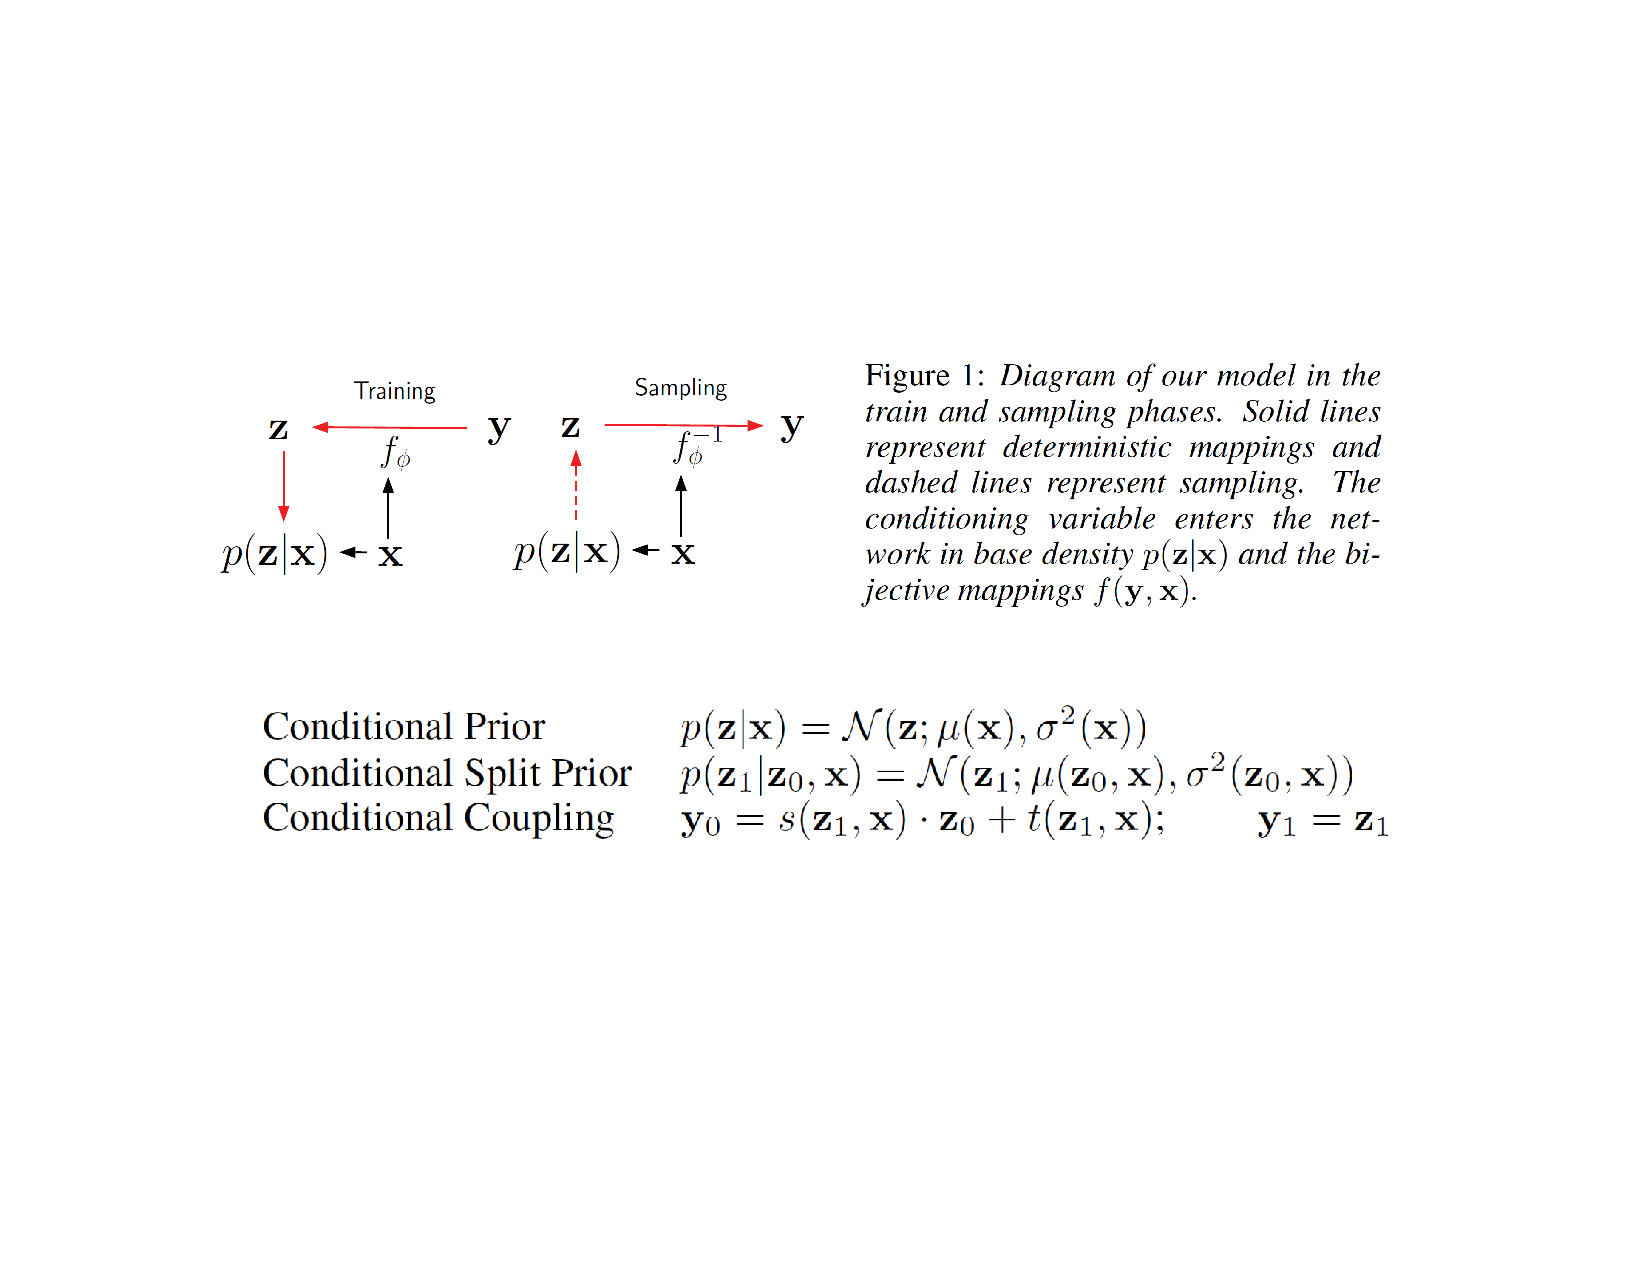
\includegraphics[width=0.8\textwidth]{../figures/cnf.pdf}
    \caption{The diagram of CNFs}
\end{figure}
\end{frame}

\begin{frame}{CNFs: How to Condition \& Build the Flow}
\textbf{Condition injection:}
\begin{align*}
\text{Conditional prior: } & p(\mathbf{z}\mid \mathbf{x})=\mathcal{N}\!\big(\mu(\mathbf{x}), \operatorname{diag}\sigma^2(\mathbf{x})\big).\\
\text{Coupling (affine): } &
\begin{cases}
\mathbf{y}_a = \mathbf{z}_a, \\
\mathbf{y}_b = \mathbf{z}_b \odot \exp s(\mathbf{z}_a,\mathbf{x}) + t(\mathbf{z}_a,\mathbf{x}),
\end{cases}
\quad\Rightarrow\quad \log|\det J|=\sum s(\mathbf{z}_a,\mathbf{x}).
\end{align*}

\medskip
\textbf{Architecture primitives:}
\begin{itemize}
  \item \emph{Coupling layers} (additive/affine/rational-quadratic spline) for cheap Jacobians.
  \item \emph{Invertible $1{\times}1$ convs} or permutations to mix channels.
  \item \emph{Multi-scale} (squeeze \& factor-out) for efficiency and expressivity.
\end{itemize}

\medskip
\textbf{Implementation pattern.} Encode $\mathbf{x}$ once: $\mathbf{h}=g(\mathbf{x})$; pass $\mathbf{h}$ to all conditioner nets (those producing $s,t,\mu,\sigma$) via concatenation or FiLM/AdaIN-style modulation.
\end{frame}

\begin{frame}{CNFs: Design Choices, Tips, \& When to Use CNFs}
\textbf{Design choices.}
\begin{itemize}
  \item \emph{Base} $p(\mathbf{z}\mid\mathbf{x})$: diagonal Gaussian (fast) vs.\ low-rank covariance (richer).
  \item \emph{Coupling type}: additive (stable), affine (scales variance), spline (captures sharp changes).
  \item \emph{Conditioning nets}: small MLP/CNN/Transformer; use weight norm/actnorm for stability.
\end{itemize}

\textbf{Training tips.}
\begin{itemize}
  \item Minibatch NLL with EMA of actnorm stats; gradient clipping for deep flows.
  \item Warm up the scale in affine/spline couplings (e.g., $s\!\leftarrow\!\tanh(\cdot)$ or scaled output).
  \item Multi-scale factor-out improves likelihood and sampling speed.
\end{itemize}

\textbf{Why CNFs vs.\ alternatives?}
\begin{itemize}
  \item \emph{Exact} conditional likelihood (useful for evaluation \& downstream scoring).
  \item Faster sampling than diffusion; richer joint modeling than per-dimension regressions.
  \item Good fit for structured prediction where uncertainty matters (SR, optical flow, segmentation logits, etc.).
\end{itemize}
\end{frame}

\section{Training and Applications}

\begin{frame}{Maximum Likelihood Training}
Given data $\{\mathbf{x}^{(i)}\}_{i=1}^N$, maximize:
\begin{equation}
    \mathcal{L}(\theta) = \frac{1}{N} \sum_{i=1}^N \log p_\theta(\mathbf{x}^{(i)})
\end{equation}

\textbf{Gradient computation}:
\begin{equation}
    \nabla_\theta \mathcal{L} = \frac{1}{N} \sum_{i=1}^N \nabla_\theta \log p_\theta(\mathbf{x}^{(i)})
\end{equation}

\textbf{Challenges}:
\begin{itemize}
    \item \textcolor{red}{Mode collapse}: Flow might ignore some data modes
    \item \textcolor{red}{Training instability}: Gradients can be large
    \item \textcolor{red}{Computational cost}: Jacobian computation is expensive
\end{itemize}
\end{frame}

\begin{frame}{Applications of Normalizing Flows}
\textbf{Generative modeling}:
\begin{itemize}
    \item Image generation (Real NVP, Glow)
    \item Audio synthesis (WaveGlow)
    \item Text generation (FlowSeq)
\end{itemize}

\textbf{Density estimation}:
\begin{itemize}
    \item Anomaly detection
    \item Out-of-distribution detection
    \item Uncertainty quantification
\end{itemize}

\textbf{Variational inference}:
\begin{itemize}
    \item Posterior approximation
    \item Bayesian neural networks
    \item Variational autoencoders
\end{itemize}
\end{frame}



\section{Comparison with Other Methods}

\begin{frame}{Normalizing Flows vs. Other Generative Models}
\begin{table}
\centering
\begin{tabular}{|l|c|c|c|c|}
\hline
Method & Exact Likelihood & Fast Sampling & Fast Training & Stable \\
\hline
VAE & \textcolor{red}{No} & \textcolor{green}{Yes} & \textcolor{green}{Yes} & \textcolor{green}{Yes} \\
GAN & \textcolor{red}{No} & \textcolor{green}{Yes} & \textcolor{red}{No} & \textcolor{red}{No} \\
Diffusion & \textcolor{red}{No} & \textcolor{red}{No} & \textcolor{green}{Yes} & \textcolor{green}{Yes} \\
Normalizing Flow & \textcolor{green}{Yes} & \textcolor{green}{Yes} & \textcolor{red}{No} & \textcolor{green}{Yes} \\
\hline
\end{tabular}
\end{table}

\textbf{Unique advantages of Normalizing Flows}:
\begin{itemize}
    \item \textcolor{blue}{Exact likelihood}: Can compute $p(x)$ exactly
    \item \textcolor{blue}{Exact sampling}: Can generate samples exactly
    \item \textcolor{blue}{Latent space}: Natural representation learning
    \item \textcolor{blue}{Interpretability}: Understandable transformations
\end{itemize}
\end{frame}

\section{Challenges and Future Directions}

\begin{frame}{Current Challenges}
\textbf{Computational challenges}:
\begin{itemize}
    \item \textcolor{red}{Jacobian computation}: Expensive for high dimensions
    \item \textcolor{red}{Memory usage}: Need to store intermediate states
    \item \textcolor{red}{Training time}: Slower than GANs or VAEs
\end{itemize}

\textbf{Modeling challenges}:
\begin{itemize}
    \item \textcolor{red}{Architectural constraints}: Must be invertible
    \item \textcolor{red}{Mode collapse}: May ignore some data modes
    \item \textcolor{red}{Expressiveness}: Limited by transformation family
\end{itemize}

\textbf{Theoretical challenges}:
\begin{itemize}
    \item \textcolor{red}{Universal approximation}: Not guaranteed for all distributions
    \item \textcolor{red}{Convergence}: No global convergence guarantees
    \item \textcolor{red}{Generalization}: Limited theoretical understanding
\end{itemize}
\end{frame}

\begin{frame}{Future Directions}
\textbf{Architectural improvements}:
\begin{itemize}
    \item \textcolor{blue}{More flexible transformations}: Beyond coupling layers
    \item \textcolor{blue}{Better conditioning}: Improved numerical stability
    \item \textcolor{blue}{Efficient computation}: Faster Jacobian computation
\end{itemize}

\textbf{Training improvements}:
\begin{itemize}
    \item \textcolor{blue}{Better optimization}: More stable training
    \item \textcolor{blue}{Regularization}: Prevent overfitting
    \item \textcolor{blue}{Multi-scale training}: Progressive complexity
\end{itemize}

\textbf{Applications}:
\begin{itemize}
    \item \textcolor{blue}{High-dimensional data}: Images, videos, audio
    \item \textcolor{blue}{Scientific computing}: Physics simulations
    \item \textcolor{blue}{Robotics}: Motion planning and control
\end{itemize}
\end{frame}

\section{Conclusion}

\begin{frame}{Summary}
\textbf{Normalizing flows provide}:
\begin{itemize}
    \item \textcolor{green}{Exact likelihood computation}
    \item \textcolor{green}{Exact sampling}
    \item \textcolor{green}{Flexible architectures}
    \item \textcolor{green}{Interpretable representations}
\end{itemize}

\textbf{Key insights}:
\begin{itemize}
    \item \textcolor{blue}{Change of variables}: Foundation of all flow-based methods
    \item \textcolor{blue}{Jacobian computation}: Central computational challenge
    \item \textcolor{blue}{Architectural design}: Balance between expressiveness and efficiency
    \item \textcolor{blue}{Training strategies}: Maximum likelihood with proper regularization
\end{itemize}

\textbf{Future work}:
\begin{itemize}
    \item \textcolor{red}{Scalability}: Handle higher-dimensional data
    \item \textcolor{red}{Efficiency}: Reduce computational costs
    \item \textcolor{red}{Theoretical understanding}: Better convergence guarantees
\end{itemize}
\end{frame}

% Thank you slide  
\begin{frame}{Welcome inputs}  
  \centering  
  Any comments?
  \\[2em]
  Welcome your inputs!  
\end{frame}  
  
\end{document}
